\PassOptionsToPackage{unicode=true}{hyperref} % options for packages loaded elsewhere
\PassOptionsToPackage{hyphens}{url}
%
\documentclass[12pt,]{article}
\usepackage{lmodern}
\usepackage{amssymb,amsmath}
\usepackage{ifxetex,ifluatex}
\usepackage{fixltx2e} % provides \textsubscript
\ifnum 0\ifxetex 1\fi\ifluatex 1\fi=0 % if pdftex
  \usepackage[T1]{fontenc}
  \usepackage[utf8]{inputenc}
  \usepackage{textcomp} % provides euro and other symbols
\else % if luatex or xelatex
  \usepackage{unicode-math}
  \defaultfontfeatures{Ligatures=TeX,Scale=MatchLowercase}
\fi
% use upquote if available, for straight quotes in verbatim environments
\IfFileExists{upquote.sty}{\usepackage{upquote}}{}
% use microtype if available
\IfFileExists{microtype.sty}{%
\usepackage[]{microtype}
\UseMicrotypeSet[protrusion]{basicmath} % disable protrusion for tt fonts
}{}
\IfFileExists{parskip.sty}{%
\usepackage{parskip}
}{% else
\setlength{\parindent}{0pt}
\setlength{\parskip}{6pt plus 2pt minus 1pt}
}
\usepackage{hyperref}
\hypersetup{
            pdfborder={0 0 0},
            breaklinks=true}
\urlstyle{same}  % don't use monospace font for urls
\usepackage[margin=2.5cm,hoffset=1.5cm,a4paper]{geometry}
\usepackage{graphicx,grffile}
\makeatletter
\def\maxwidth{\ifdim\Gin@nat@width>\linewidth\linewidth\else\Gin@nat@width\fi}
\def\maxheight{\ifdim\Gin@nat@height>\textheight\textheight\else\Gin@nat@height\fi}
\makeatother
% Scale images if necessary, so that they will not overflow the page
% margins by default, and it is still possible to overwrite the defaults
% using explicit options in \includegraphics[width, height, ...]{}
\setkeys{Gin}{width=\maxwidth,height=\maxheight,keepaspectratio}
\setlength{\emergencystretch}{3em}  % prevent overfull lines
\providecommand{\tightlist}{%
  \setlength{\itemsep}{0pt}\setlength{\parskip}{0pt}}
\setcounter{secnumdepth}{0}
% Redefines (sub)paragraphs to behave more like sections
\ifx\paragraph\undefined\else
\let\oldparagraph\paragraph
\renewcommand{\paragraph}[1]{\oldparagraph{#1}\mbox{}}
\fi
\ifx\subparagraph\undefined\else
\let\oldsubparagraph\subparagraph
\renewcommand{\subparagraph}[1]{\oldsubparagraph{#1}\mbox{}}
\fi

% set default figure placement to htbp
\makeatletter
\def\fps@figure{htbp}
\makeatother


\date{}

\begin{document}

\hypertarget{concentradores}{%
\section{Concentradores}\label{concentradores}}

Calculo de extracción Solido-líquido. (Procedimiento)
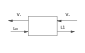
\includegraphics{./tex2pdf.4952/0fb63f1303abfee3a97089307b3d8e0ecbe65cb3.svg}
\#\#\#\# 1. Cálculo de \(X_M\)
\textgreater{}\(X_{SM} = \frac{(L_0 X_{S0} + V_2 Y_{S2})}{ (L_0 + V_2)}\)

\begin{quote}
\(X_{AM} = \frac{(L_0 X_{A0} + V_2 Y_{A2})}{(L_0+V_2)}\)
\end{quote}

\begin{quote}
\(X_M=[X_{SM},X_{AM}]\)
\end{quote}

\hypertarget{cuxe1lculo-de-x_1}{%
\paragraph{\texorpdfstring{2. Cálculo de
\(X_1\)}{2. Cálculo de X\_1}}\label{cuxe1lculo-de-x_1}}

\begin{quote}
\(\frac{X_{SM}}{X_{AM}} X_{A1}=X_S-X_{A1}\)
\end{quote}

\begin{quote}
\(X_S -X_{A1} -X_{SM}/X_{AM}X_{A1}\)
\end{quote}

\begin{quote}
\(-X_S = -X_{A1}(1+\frac{X_{SM}}{X_{AM}})\)
\end{quote}

\begin{quote}
\(X_{A1} = \frac{X_S}{(1+X_{SM}/X_{AM})}\)
\end{quote}

\begin{quote}
\(X_{S1} = 1-X_B - X_{A1}\)
\end{quote}

\begin{quote}
\(X_1 = [X_{A1},X_{S1}]\)
\end{quote}

\hypertarget{cuxe1lculo-de-y_1}{%
\paragraph{\texorpdfstring{3. Cálculo de
\(Y_1\)}{3. Cálculo de Y\_1}}\label{cuxe1lculo-de-y_1}}

\begin{quote}
\(\frac{X_{SM}}{X_{AM}} Y_{A1}=Y_S- \frac{Y_{S2}}{X_{A0}}Y_{A1}\)
\end{quote}

\begin{quote}
\((\frac{Y_{S2}}{X_{A0}}+\frac{X_{SM}}{X_{AM}}) Y_{A1}=Y_S\)
\end{quote}

\begin{quote}
\(Y_{A1}=\frac{Y_S}{(\frac{Y_{S2}}{X_{A0}}+\frac{X_{SM}}{X_{AM}})}\)
\end{quote}

\begin{quote}
\(Y_{S1}=1-Y_{A1}\)
\end{quote}

\begin{quote}
\(Y_1=[Y_{A1},Y_{S1}]\)
\end{quote}

\end{document}
